% Use figure* for multi-column figure

\begin{figure}[tp]
  \centering
  \begin{subfigure}{0.45\textwidth}
    \centering
    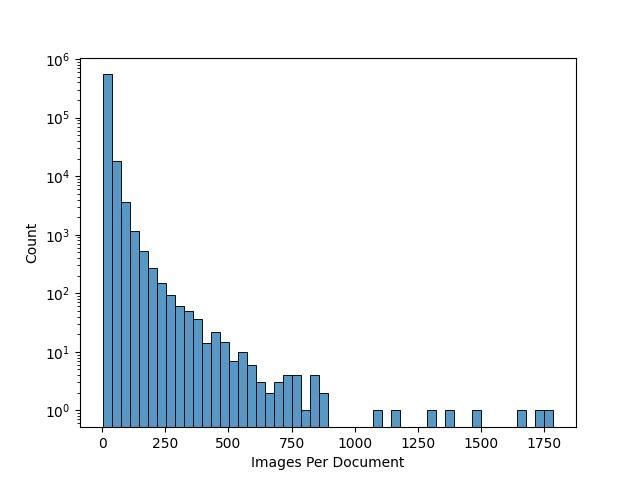
\includegraphics[width=\textwidth]{figs/data-statistic/n_images_by_paper.jpg}
    \caption{Image Number Distribution over Paper.}
    \label{fig:subfig1}
  \end{subfigure}
  % \hfill
  % \begin{subfigure}{0.45\textwidth}
  %   \centering
  %   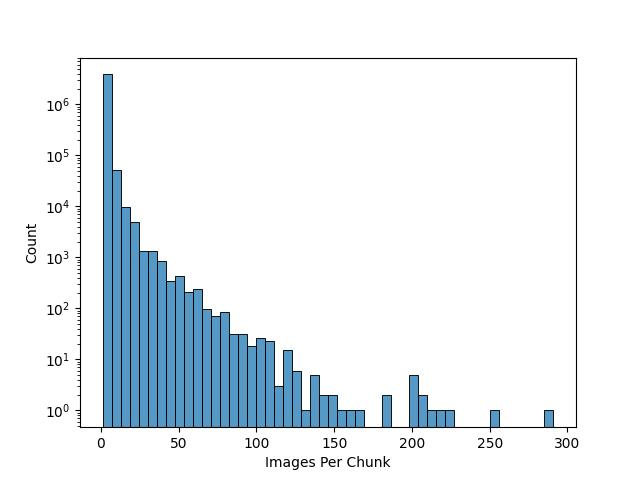
\includegraphics[width=\textwidth]{figs/data-statistic/n_images_by_block.jpg}
  %   \caption{Image Number Distribution over Block.}
  %   \label{fig:subfig2}
  % \end{subfigure}
  \hfill
  % \begin{subfigure}{0.45\textwidth}
  %   \centering
  %   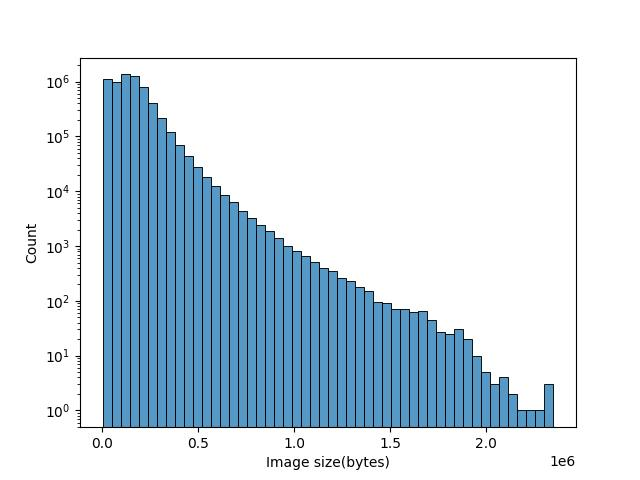
\includegraphics[width=\textwidth]{figs/data-statistic/image_sizes.jpg}
  %   \caption{Image Size Distribution.}
  %   \label{fig:subfig2}
  % \end{subfigure}
  \caption{Image Statistic.}
  \label{fig:image-statistic}
\end{figure}